\documentclass[11pt,a4paper]{article}
\usepackage[utf8]{inputenc}
\usepackage[vietnamese]{babel}
\usepackage{amsmath,amssymb}
\usepackage[version=4]{mhchem}
\usepackage{geometry}
\geometry{top=0.65cm,bottom=0.65cm,left=1.25cm,right=1.25cm,headheight=20pt,headsep=3pt,footskip=9pt}
\usepackage{graphicx}
\usepackage{xcolor}
\usepackage{tabularx}
\usepackage{array}
\usepackage{tikz}
\usepackage{multicol}
\usepackage{fancyhdr}
\usepackage{enumitem}

\definecolor{hfRed}{HTML}{D32F2F}
\definecolor{hfGreen}{HTML}{8BC390}
\definecolor{mainGreen}{HTML}{2E7D32}

\usepackage{ex_test}

\pagestyle{fancy}
\fancyhf{}
\renewcommand{\headrulewidth}{0.75pt}
\renewcommand{\headrule}{\hbox to\headwidth{\color{hfGreen}\leaders\hrule height \headrulewidth\hfill}}
\renewcommand{\footrulewidth}{0.75pt}
\renewcommand{\footrule}{\hbox to\headwidth{\color{hfGreen}\leaders\hrule height \footrulewidth\hfill}}

\fancyhead[L]{\small\itshape\color{hfRed}Tài liệu lưu hành nội bộ}
\fancyhead[R]{\small\color{hfRed}Thầy \textbf{TRẦN VĂN THẠNH} - 0777.470.803}

\fancyfoot[L]{\footnotesize\itshape\color{hfRed}CS1: 6/15 Nguyễn Hoàng, P. Kim Long, TP Huế \quad|\quad CS2: 24 Đặng Thái Thân, TP Huế}
\fancyfoot[R]{\small\textbf{\color{hfRed}Trang \thepage}}

\setlength{\parindent}{0pt}
\setlength{\parskip}{1.0pt}

\def\loigiai#1{
\par\begingroup\color{blue!80!black}\small
\noindent\textbf{\textit{Lời giải chi tiết:}}\par
#1\par\endgroup}

\begin{document}
\Opensolutionfile{ans}[ans-de21-gv]

\noindent
\begin{minipage}[t]{0.48\textwidth}
	\textbf{SỞ GIÁO DỤC VÀ ĐÀO TẠO THỪA THIÊN HUẾ}\\
	\textbf{TRƯỜNG THPT HAI BÀ TRƯNG}\\
	\textbf{ĐỀ CHÍNH THỨC}\\
	\textit{(Đề thi có 04 trang)}
\end{minipage}\hfill
\begin{minipage}[t]{0.48\textwidth}
	\raggedleft
	\textbf{\color{mainGreen}ĐỀ KIỂM TRA ĐỊNH KỲ CHƯƠNG 7 (KIM LOẠI NHÓM IA \& IIA)}\\
	\textbf{MÔN: HOÁ HỌC -- LỚP 12}\\
	\textit{Thời gian làm bài: 50 phút (không kể thời gian phát đề)}\\
	\textbf{Mã đề thi: 121}
\end{minipage}


\vspace{0.1cm}
\begin{center}
	\textbf{\color{hfRed}\Large (BẢN GIÁO VIÊN -- CÓ LỜI GIẢI CHI TIẾT)}
\end{center}

\vspace{1pt}
\noindent\textit{Họ, tên thí sinh: \dots\dots\dots\dots\dots\dots\dots\dots\dots\dots\dots\dots\dots\dots\dots\dots\dots\dots\dots\dots\dots\dots Lớp: \dots\dots\dots\dots SBD: \dots\dots\dots\dots}\\
\noindent\textit{(Cho biết nguyên tử khối: H = 1; C = 12; N = 14; O = 16; Na = 23; Mg = 24; Al = 27; P = 31; S = 32; Cl = 35,5; K = 39; Ca = 40; Fe = 56; Cu = 64; Zn = 65; Br = 80; Rb = 85,5; Ag = 108; Cs = 133; Ba = 137).}

\vspace{1pt}
\noindent
\textbf{PHẦN I (4,5 điểm -- 18 câu): Câu trắc nghiệm nhiều phương án lựa chọn.}\\
\textit{Thí sinh trả lời từ câu 1 đến câu 18. Mỗi câu hỏi thí sinh chỉ chọn một phương án.}

\begin{ex}
Chất nào sau đây tác dụng được với dung dịch \ce{KHCO3}?
\choice
{\ce{K2SO4}.}
{\ce{KNO3}.}
{\True \ce{HCl}.}
{\ce{KCl}.}
\loigiai{
$\ce{KHCO3 + HCl -> KCl + CO2 ^ + H2O}$.\\
\textbf{Chọn C.}}
\end{ex}

\begin{ex}
Dung dịch \ce{Na2CO3} tác dụng được với dung dịch nào sau đây?
\choice
{\ce{Na2SO4}.}
{\ce{KNO3}.}
{\ce{KOH}.}
{\True \ce{CaCl2}.}
\loigiai{
$\ce{Na2CO3 + CaCl2 -> CaCO3 v + 2NaCl}$.\\
\textbf{Chọn D.}}
\end{ex}

\begin{ex}
Dung dịch nào sau đây phản ứng với dung dịch \ce{HCl} dư tạo ra chất khí?
\choice
{\ce{Ba(OH)2}.}
{\True \ce{Na2CO3}.}
{\ce{K2SO4}.}
{\ce{Ca(NO3)2}.}
\loigiai{
$\ce{Na2CO3 + 2HCl -> 2NaCl + CO2 ^ + H2O}$.\\
\textbf{Chọn B.}}
\end{ex}

\begin{ex}
Trong cốc nước chứa 0,01 mol \ce{Na+}; 0,02 mol \ce{Ca^2+}; 0,01 mol \ce{Mg^2+}; 0,05 mol \ce{HCO3-} và 0,02 mol \ce{Cl-}. Đun sôi cốc nước hồi lâu, nước thu được là
\choice
{Nước cứng tạm thời.}
{\True Nước cứng vĩnh cửu.}
{Nước mềm.}
{Nước cứng toàn phần.}
\loigiai{
Khi đun sôi: $\ce{2HCO3- -> CO3^2- + CO2 ^ + H2O} \rightarrow n_{\ce{CO3^2-}} = 0{,}025\text{ mol}$.\\
$\ce{Ca^2+ + CO3^2- -> CaCO3 v}$ (hết 0,02 mol \ce{Ca^2+} và 0,02 mol \ce{CO3^2-}).\\
$\ce{Mg^2+ + CO3^2- -> MgCO3 v}$ (kết tủa 0,005 mol \ce{Mg^2+}, còn dư 0,005 mol \ce{Mg^2+}).\\
Sau khi đun sôi, nước còn chứa 0,005 mol \ce{Mg^2+} và 0,02 mol \ce{Cl-}, không còn \ce{HCO3-} $\rightarrow$ Nước cứng vĩnh cửu.\\
\textbf{Chọn B.}}
\end{ex}

\begin{ex}
Phản ứng giải thích sự hình thành thạch nhũ trong các hang động núi đá vôi là:
\choice
{$\ce{CaCO3 + CO2 + H2O -> Ca(HCO3)2}$.}
{$\ce{CaCO3 + 2HCl -> CaCl2 + CO2 + H2O}$.}
{$\ce{CaCO3 ->[t^\circ] CaO + CO2}$.}
{\True $\ce{Ca(HCO3)2 <=> CaCO3 + CO2 + H2O}$.}
\loigiai{
Phản ứng tạo thạch nhũ: $\ce{Ca(HCO3)2 -> CaCO3 v + CO2 ^ + H2O}$.\\
\textbf{Chọn D.}}
\end{ex}

\begin{ex}
Nước thải công nghiệp thường chứa các ion kim loại nặng như \ce{Hg^2+}, \ce{Pb^2+}, \ce{Fe^3+}. Để xử lí triệt để và làm giảm nồng độ của các ion kim loại nặng với chi phí thấp nhất, người ta sử dụng dung dịch chất nào sau đây?
\choice
{\ce{HCl}.}
{\ce{NaCl}.}
{\True \ce{Ca(OH)2}.}
{\ce{K2SO4}.}
\loigiai{
Nước vôi \ce{Ca(OH)2} rẻ tiền, tạo kết tủa hydroxide/oxit với các ion kim loại nặng để lọc bỏ.\\
\textbf{Chọn C.}}
\end{ex}

\begin{ex}
Cho các dãy kim loại sau: Fe, Na, K, Cu và Li. Số kim loại trong dãy tác dụng được với nước ở nhiệt độ thường là
\choice
{1.}
{2.}
{\True 3.}
{4.}
\loigiai{
Có 3 kim loại là Na, K, Li tác dụng với nước ở nhiệt độ thường.\\
\textbf{Chọn C.}}
\end{ex}

\begin{ex}
Nguyên tắc cơ bản để làm mềm nước cứng là làm giảm nồng độ của
\choice
{\True ion \ce{Ca^2+}, \ce{Mg^2+}.}
{ion \ce{HCO3-}.}
{ion \ce{OH-}, \ce{SO4^2-}.}
{ion \ce{Ca^2+}.}
\loigiai{
Tính cứng do \ce{Ca^2+} và \ce{Mg^2+} gây ra nên nguyên tắc làm mềm nước là làm giảm nồng độ hai ion này.\\
\textbf{Chọn A.}}
\end{ex}

\begin{ex}
Kim loại nhóm IIA có nhiệt độ nóng chảy, nhiệt độ sôi, khối lượng riêng biến đổi không theo quy luật như kim loại kiềm nhóm IA, nguyên nhân chủ yếu là do các kim loại nhóm IIA có
\choice
{điện tích hạt nhân khác nhau.}
{cấu hình electron khác nhau.}
{bán kính nguyên tử khác nhau.}
{\True kiểu mạng tinh thể khác nhau.}
\loigiai{
Kim loại nhóm IIA có cấu trúc mạng tinh thể khác nhau (Be, Mg: lục phương; Ca, Sr: lập phương tâm diện; Ba: lập phương tâm khối).\\
\textbf{Chọn D.}}
\end{ex}



\begin{ex}
Khi để vôi sống trong không khí ẩm một thời gian sẽ có hiện tượng một phần bị chuyển hoá trở lại thành đá vôi. Khí nào sau đây có trong không khí gây ra hiện tượng trên?
\choice
{Oxygen.}
{Methane.}
{Nitrogen.}
{\True Carbon dioxide.}
\loigiai{
$\ce{CaO + H2O -> Ca(OH)2}$; sau đó $\ce{Ca(OH)2 + CO2 -> CaCO3 v + H2O}$. Khí gây ra là \ce{CO2}.\\
\textbf{Chọn D.}}
\end{ex}

\begin{ex}
Đun nóng tinh thể \ce{CaF2} với dung dịch \ce{H2SO4} đặc ở nhiệt độ khoảng $250^\circ\text{C}$, thu được khí nào sau đây?
\choice
{\ce{SO2}.}
{\ce{F2}.}
{\True \ce{HF}.}
{\ce{H2S}.}
\loigiai{
$\ce{CaF2 + H2SO4\text{ (đặc)} ->[250^\circ\text{C}] CaSO4 + 2HF ^}$.\\
\textbf{Chọn C.}}
\end{ex}

\begin{ex}
Cho dung dịch \ce{HCl} vào dung dịch X thấy có hiện tượng sủi bọt khí; nếu cho dung dịch \ce{Ca(OH)2} vào dung dịch X thì sinh ra kết tủa trắng. Dung dịch X là
\choice
{\ce{Na2SO4}.}
{\ce{KNO3}.}
{\True \ce{Ca(HCO3)2}.}
{\ce{BaCl2}.}
\loigiai{
$\ce{Ca(HCO3)2 + 2HCl -> CaCl2 + 2CO2 ^ + 2H2O}$;\\
$\ce{Ca(HCO3)2 + Ca(OH)2 -> 2CaCO3 v + 2H2O}$.\\
\textbf{Chọn C.}}
\end{ex}

\begin{ex}
Cho một mẩu Na vào dung dịch \ce{MgSO4} dư, thu được kết tủa X và chất khí Y. Hai chất X, Y lần lượt là
\choice
{Mg và \ce{H2}.}
{\True \ce{Mg(OH)2} và \ce{H2}.}
{Mg và \ce{O2}.}
{\ce{Na2SO4} và \ce{H2}.}
\loigiai{
$\ce{2Na + 2H2O -> 2NaOH + H2 ^}$ (khí Y là \ce{H2});\\
$\ce{2NaOH + MgSO4 -> Mg(OH)2 v + Na2SO4}$ (kết tủa X là \ce{Mg(OH)2}).\\
\textbf{Chọn B.}}
\end{ex}

\begin{ex}
Trong cốc nước chứa nhiều các ion sau: \ce{Ca^2+}, \ce{Mg^2+}, \ce{Cl-}, \ce{SO4^2-}. Nước trong cốc trên thuộc loại
\choice
{\True có tính cứng vĩnh cửu.}
{không có tính cứng.}
{có tính cứng tạm thời.}
{có tính cứng toàn phần.}
\loigiai{
Nước chứa \ce{Ca^2+}, \ce{Mg^2+}, \ce{Cl-}, \ce{SO4^2-} là nước có tính cứng vĩnh cửu.\\
\textbf{Chọn A.}}
\end{ex}

\begin{ex}
Nhận định nào \textbf{không} đúng về cấu tạo và tính chất của các kim loại nhóm IIA?
\choice
{Khối lượng riêng tương đối nhỏ, là những kim loại nhẹ hơn nhôm (trừ Ba).}
{Độ cứng cao hơn kim loại nhóm IA, nhưng mềm hơn kim loại nhôm.}
{\True Mạng tinh thể của chúng đều có kiểu lập phương tâm khối.}
{Nhiệt độ nóng chảy và nhiệt độ sôi tương đối thấp (trừ Be).}
\loigiai{
Kim loại nhóm IIA có các kiểu mạng khác nhau: Be, Mg lục phương; Ca, Sr lập phương tâm diện; Ba lập phương tâm khối.\\
\textbf{Chọn C.}}
\end{ex}

\begin{ex}
Cho các nhận định sau về tác hại của nước cứng:\\
(1) Làm giảm bọt và giảm khả năng tẩy rửa khi giặt quần áo bằng xà phòng.\\
(2) Làm đường ống dẫn nước bị đóng cặn, giảm lưu lượng dòng chảy.\\
(3) Làm thức ăn lâu chín và giảm mùi vị đặc trưng khi nấu nướng.\\
(4) Làm nồi hơi bị phủ cặn cách nhiệt, gây tốn nhiên liệu và có nguy cơ gây nổ lò hơi.\\
Số nhận định đúng là
\choice
{1.}
{2.}
{3.}
{\True 4.}
\loigiai{
Cả 4 nhận định trên đều đúng.\\
\textbf{Chọn D.}}
\end{ex}

\begin{ex}
Phát biểu nào sau đây \textbf{không} đúng?
\choice
{Đun sôi nước cứng chỉ làm mềm nước cứng tạm thời.}
{Dung dịch \ce{Na2CO3} làm mềm nước cứng tạm thời, nước cứng vĩnh cửu.}
{\True Dung dịch \ce{NH4Cl} làm mềm nước cứng.}
{Cho dung dịch \ce{Ca(OH)2} vừa đủ làm mềm nước cứng tạm thời.}
\loigiai{
Dung dịch \ce{NH4Cl} không kết tủa \ce{Ca^2+} hay \ce{Mg^2+} nên không làm mềm nước cứng.\\
\textbf{Chọn C.}}
\end{ex}

\begin{ex}
Cho sơ đồ chuyển hoá hoá học sau:
\par\vspace{1pt}\centerline{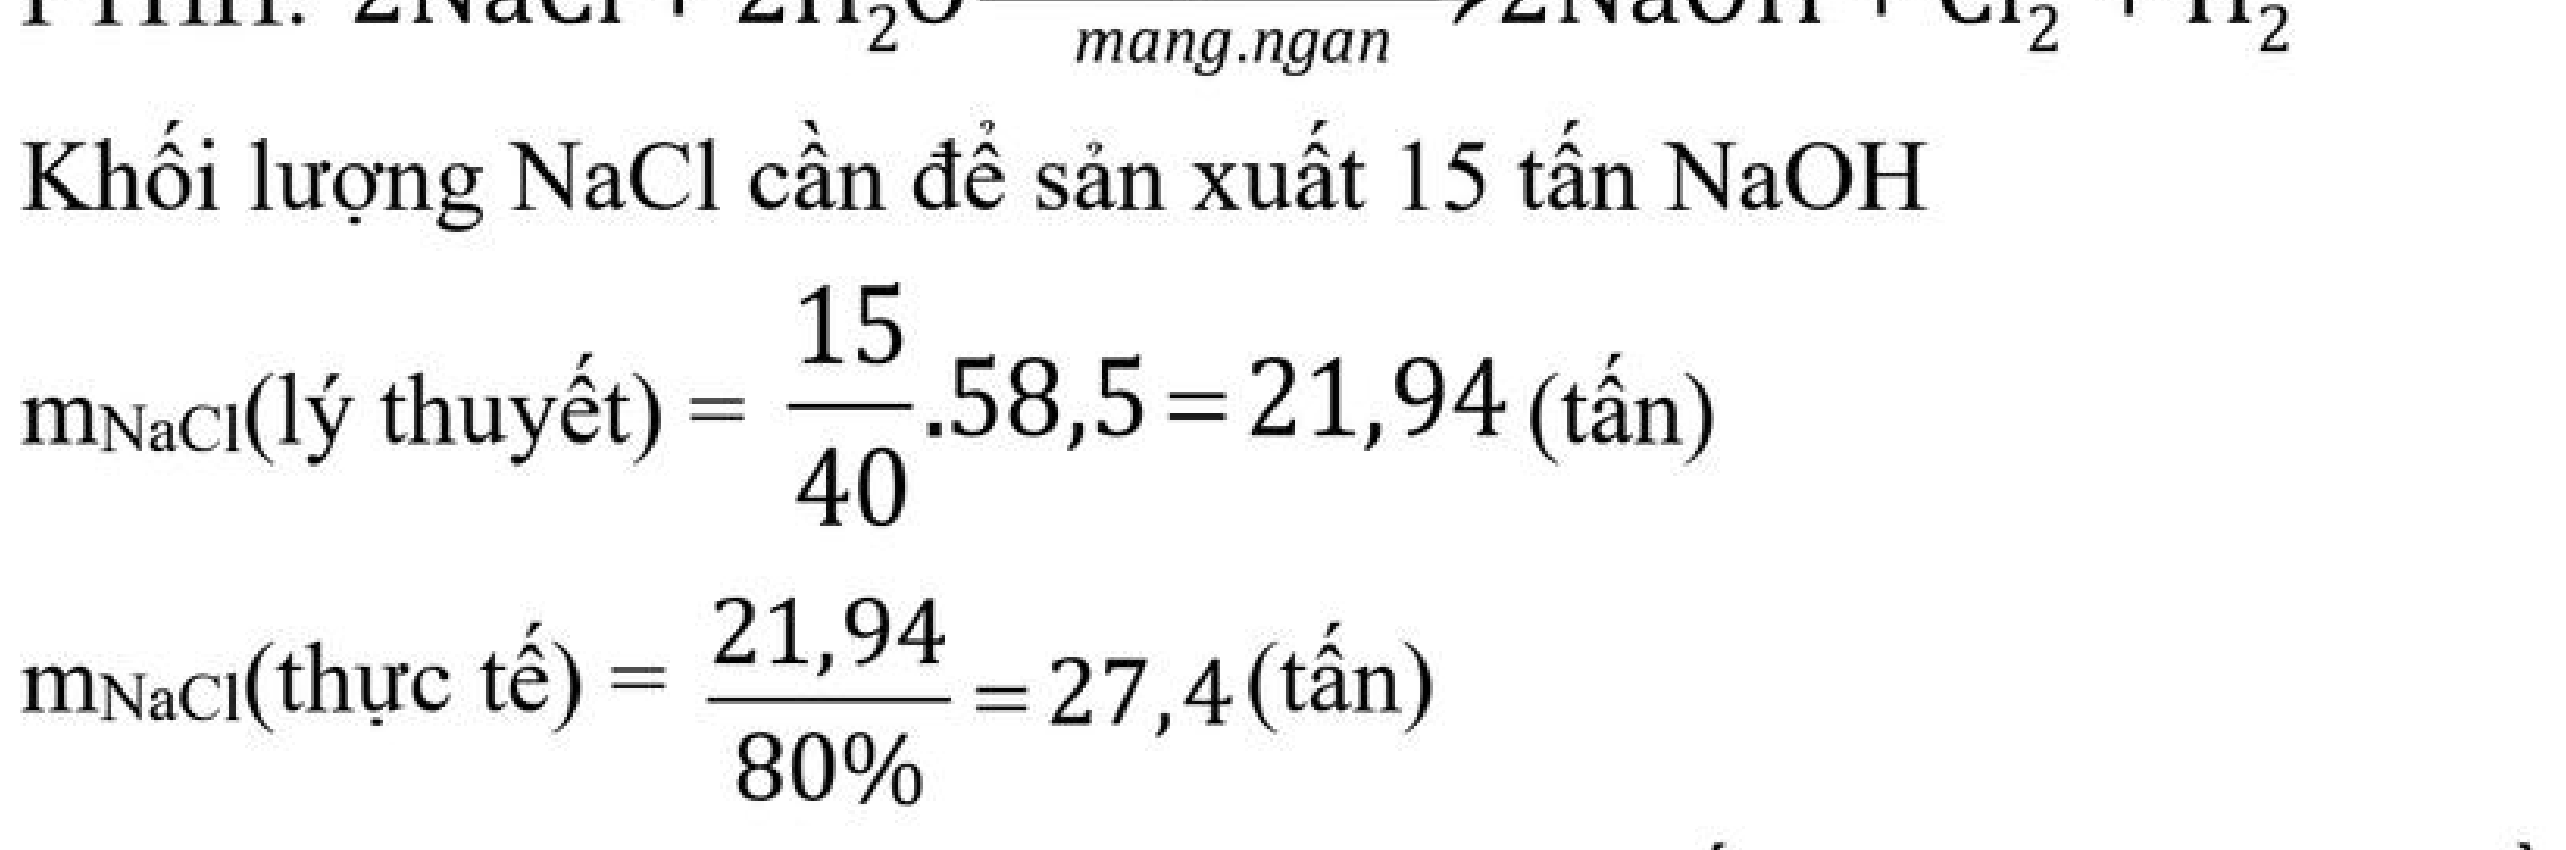
\includegraphics[height=1.45cm]{images_crop_de21/p1_cau18_so_do.png}}\vspace{1pt}
Chất X trong sơ đồ trên có thể là
\choice
{\True \ce{BaCO3}.}
{\ce{CaCO3}.}
{\ce{BaSO3}.}
{\ce{MgCO3}.}
\loigiai{
X là \ce{BaCO3}:\\
$\ce{BaCO3 ->[t^\circ] BaO (B_1) + CO2 (A_1)}$;\\
$\ce{CO2 + Ca(OH)2 -> CaCO3 v (A_2) + H2O}$; $\ce{CaCO3 ->[900^\circ\text{C}] CaO + CO2}$;\\
$\ce{BaO + 2HCl -> BaCl2 (B_2) + H2O}$; $\ce{BaCl2 + Na2SO4 -> BaSO4 v (B_3) + 2NaCl}$.\\
\textbf{Chọn A.}}
\end{ex}



\noindent
\textbf{PHẦN II (4,0 điểm -- 4 câu): Câu trắc nghiệm đúng sai.}\\
\textit{Thí sinh trả lời từ câu 1 đến câu 4. Trong mỗi ý a), b), c), d) ở mỗi câu, thí sinh chọn đúng hoặc sai.}

\setcounter{ex}{0}

\begin{ex}
Trong tự nhiên, các nguyên tố nhóm IA chỉ tồn tại ở dạng hợp chất (chủ yếu là dạng muối). Sodium và potassium là hai nguyên tố phổ biến trong vỏ Trái Đất, có nhiều trong nước biển, muối mỏ, quặng halite (\ce{NaCl}), quặng sylvinite (\ce{NaCl.KCl}).
\choiceTF
{\True Trong đời sống hàng ngày, sodium chloride được dùng làm gia vị, bảo quản và chế biến thực phẩm.}
{Điện phân dung dịch \ce{NaCl} bão hoà có màng ngăn điện cực được ứng dụng trong công nghiệp để sản xuất nước Javel.}
{\True Trong công nghiệp, khí chlorine được sản xuất bằng cách điện phân dung dịch muối ăn bão hoà có màng ngăn xốp.}
{\True Sodium carbonate là nguyên liệu quan trọng để sản xuất thuỷ tinh, xà phòng, bột giặt, giấy, sợi và chất tẩy rửa.}
\loigiai{
a) \textbf{Đúng}.\\
b) \textbf{Sai} vì sản xuất nước Javel bằng điện phân \textbf{không} có màng ngăn.\\
c) \textbf{Đúng}.\\
d) \textbf{Đúng}.}
\end{ex}

\begin{ex}
Khi nồng độ acid trong dịch vị dạ dày tăng cao có thể gây ra viêm loét dạ dày, tá tràng. Để giảm bớt nồng độ acid trong dịch vị dạ dày người ta thường dùng thuốc đau dạ dày có chứa thành phần chính là muối X.
\choiceTF
{Muối X là sodium bicarbonate có công thức hoá học là \ce{Na2CO3}.}
{\True Muối X còn được dùng để tạo độ xốp cho các loại bánh nướng, làm mềm thực phẩm.}
{\True Muối X bị phân huỷ khi đun nóng.}
{\True Trong công nghiệp hoá chất, muối X được sản xuất chủ yếu bằng phương pháp Solvay.}
\loigiai{
a) \textbf{Sai} vì muối X là sodium hydrogencarbonate có công thức là \ce{NaHCO3}.\\
b) \textbf{Đúng}. Bột nở làm xốp bánh.\\
c) \textbf{Đúng}. $\ce{2NaHCO3 ->[t^\circ] Na2CO3 + CO2 + H2O}$.\\
d) \textbf{Đúng}. Phương pháp Solvay tạo \ce{NaHCO3} kết tủa.}
\end{ex}

\begin{ex}
Bảng sau đây cho biết thông số một số tính chất vật lí cơ bản của các kim loại nhóm IIA:
\par\vspace{1pt}\centerline{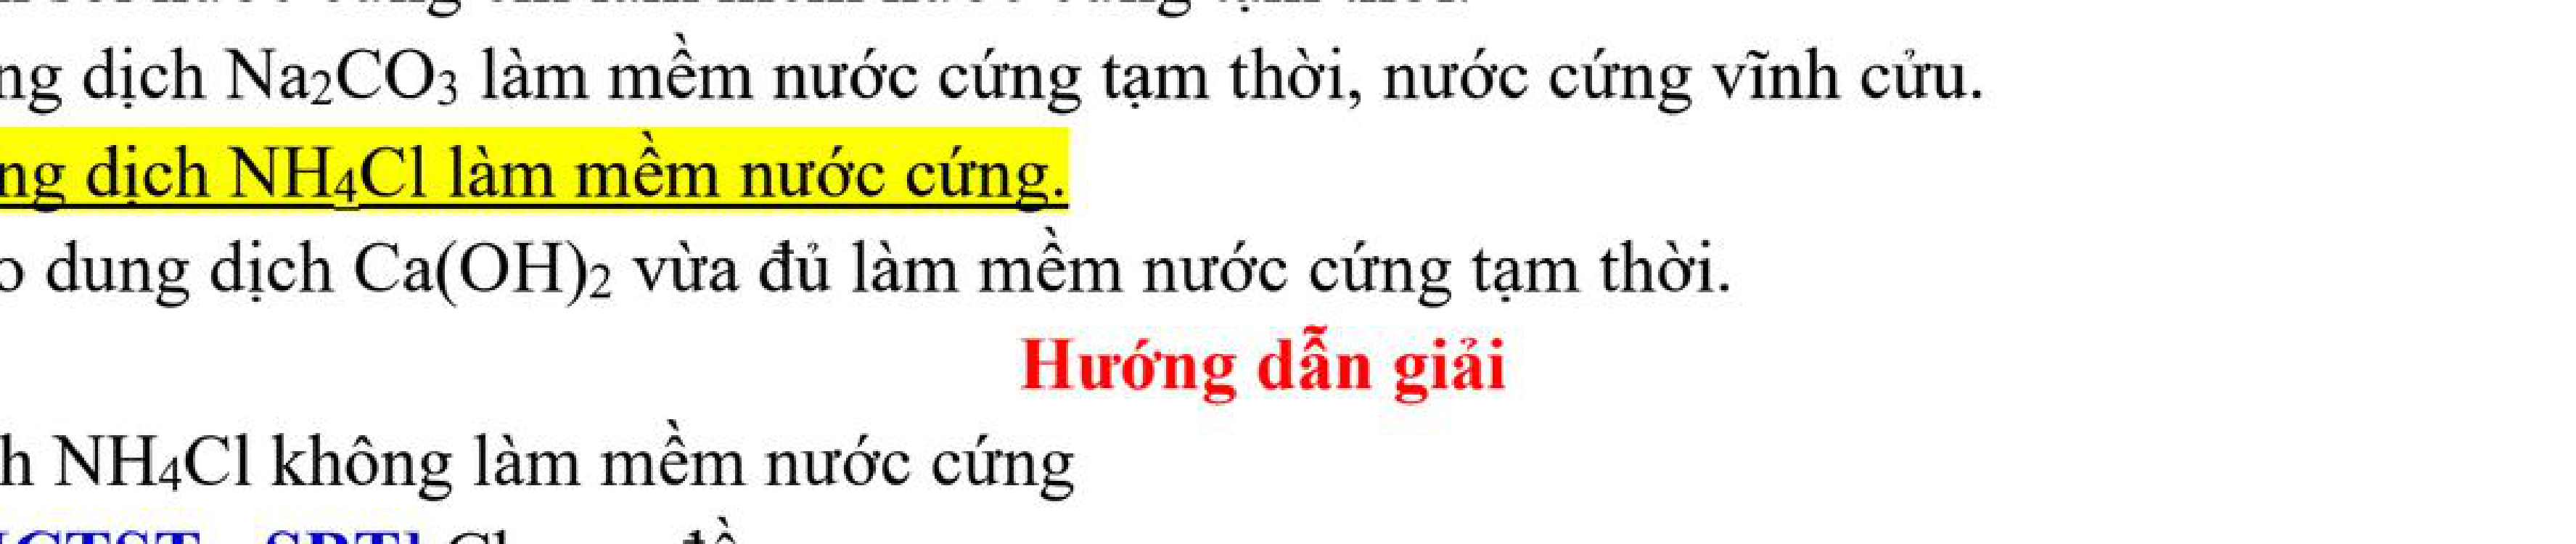
\includegraphics[height=1.5cm]{images_crop_de21/p2_cau3_bang_tinh_chat.png}}\vspace{1pt}
\choiceTF
{Nhiệt độ sôi tăng dần từ Be đến Ba.}
{Khối lượng riêng tăng dần đều đặn từ trên xuống dưới từ Mg đến Ba.}
{Độ cứng của các kim loại tăng dần từ Be đến Ba.}
{Nhiệt độ nóng chảy giảm dần đều đặn từ Be đến Ba.}
\loigiai{
a) \textbf{Sai} vì nhiệt độ sôi biến thiên không theo quy luật: 2770, 1110, 1440, 1380, 1640.\\
b) \textbf{Sai} vì khối lượng riêng không tăng đều đặn (Mg là 1,74; Ca là 1,55 g/cm$^3$).\\
c) \textbf{Sai} vì độ cứng giảm dần.\\
d) \textbf{Sai} vì nhiệt độ nóng chảy không giảm đều đặn do khác kiểu mạng tinh thể.}
\end{ex}

\begin{ex}
Cho các phản ứng hoá học xảy ra theo sơ đồ sau:\\
(1) $\ce{2X1 + 2H2O ->[dpdd, co mang ngan] 2X2 + X3 + H2}$\\
(2) $\ce{2X2 + X4 -> BaCO3 v + K2CO3 + 2H2O}$\\
(3) $\ce{X4 + X5 ->[1:1] BaSO4 v + 2CO2 ^ + 2H2O}$
\choiceTF
{\True Hợp chất $\text{X}_2$ là potassium hydroxide (KOH).}
{\True Đơn chất $\text{X}_3$ là chất khí có màu vàng lục nhạt.}
{\True Muối $\text{X}_4$ là muối acid (muối hydrogencarbonate).}
{\True Khi đun nóng dung dịch muối $\text{X}_4$ thì thu được kết tủa trắng.}
\loigiai{
$\text{X}_1$: KCl; $\text{X}_2$: KOH; $\text{X}_3$: \ce{Cl2}; $\text{X}_4$: \ce{Ba(HCO3)2}; $\text{X}_5$: \ce{H2SO4}.\\
a) \textbf{Đúng}. $\text{X}_2$ là KOH.\\
b) \textbf{Đúng}. $\text{X}_3$ là \ce{Cl2} màu vàng lục.\\
c) \textbf{Đúng}. $\text{X}_4$ là \ce{Ba(HCO3)2} (muối acid).\\
d) \textbf{Đúng}. $\ce{Ba(HCO3)2 ->[t^\circ] BaCO3 v + CO2 + H2O}$.}
\end{ex}



\noindent
\textbf{PHẦN III (1,5 điểm -- 6 câu): Câu trắc nghiệm yêu cầu trả lời ngắn.}\\
\textit{Thí sinh trả lời từ câu 1 đến câu 6.}

\setcounter{ex}{0}

\begin{ex}
Trong công nghiệp, quá trình sản xuất soda bằng phương pháp Solvay đi từ các nguyên liệu ban đầu là muối ăn (\ce{NaCl}), đá vôi (\ce{CaCO3}) và ammonia (\ce{NH3}). Có bao nhiêu phương trình hoá học chủ yếu đã xảy ra trong toàn bộ quy trình trên?
\par\noindent\textbf{Đáp số:} \textbf{\color{red}3}
\loigiai{
Có 3 phản ứng chính:\\
(1) $\ce{CaCO3 ->[t^\circ] CaO + CO2}$;\\
(2) $\ce{NaCl + NH3 + CO2 + H2O -> NaHCO3 v + NH4Cl}$;\\
(3) $\ce{2NaHCO3 ->[t^\circ] Na2CO3 + CO2 + H2O}$.\\
\textbf{Đáp số: 3.}}
\end{ex}

\begin{ex}
Cho các nguyên tố sau: Kr, Ca, Sr, Li, Ni, Rb. Có bao nhiêu nguyên tố là kim loại kiềm (nhóm IA) trong dãy trên?
\par\noindent\textbf{Đáp số:} \textbf{\color{red}2}
\loigiai{
Có 2 kim loại kiềm (nhóm IA) là Li và Rb.\\
\textbf{Đáp số: 2.}}
\end{ex}

\begin{ex}
Cho các chất sau: \ce{Ca(OH)2}, \ce{Na2CO3}, \ce{Na3PO4}, \ce{NaOH}, \ce{KCl}. Có bao nhiêu chất có thể dùng để làm mềm nước có tính cứng vĩnh cửu?
\par\noindent\textbf{Đáp số:} \textbf{\color{red}2}
\loigiai{
Có 2 chất là \ce{Na2CO3} và \ce{Na3PO4}.\\
\textbf{Đáp số: 2.}}
\end{ex}

\begin{ex}
Cho dung dịch của 4 chất sau đều trong suốt và không màu: \ce{NaCl}, \ce{Na2SO4}, \ce{KCl}, \ce{LiNO3}. Chỉ dùng ngọn lửa không màu của đèn khí thì có thể nhận biết được bao nhiêu dung dịch riêng biệt trong số 4 dung dịch trên?
\par\noindent\textbf{Đáp số:} \textbf{\color{red}2}
\loigiai{
Nhận biết được 2 dung dịch là KCl (ngọn lửa tím nhạt) và \ce{LiNO3} (ngọn lửa đỏ tía). Hai dung dịch \ce{NaCl} và \ce{Na2SO4} đều ngọn lửa vàng nên không phân biệt được với nhau.\\
\textbf{Đáp số: 2.}}
\end{ex}

\begin{ex}
Ở $20^\circ\text{C}$, độ tan của \ce{NaCl} trong nước là 35,9 gam trong 100 gam nước. Ở nhiệt độ này, dung dịch \ce{NaCl} bão hoà có nồng độ phần trăm là $a\%$. Xác định giá trị của $a$ (làm tròn kết quả đến hàng phần mười).
\par\noindent\textbf{Đáp số:} \textbf{\color{red}26,4}
\loigiai{
$C\% = \dfrac{35{,}9}{100 + 35{,}9} \times 100\% = \dfrac{35{,}9}{135{,}9} \times 100\% \approx 26{,}4\%$.\\
\textbf{Đáp số: 26,4.}}
\end{ex}

\begin{ex}
Một loại thuốc kháng acid dạ dày có tên thương mại là Rolaids chứa thành phần hoạt chất chính là dihydroxyaluminum sodium carbonate có công thức \ce{NaAl(OH)2CO3}. Mỗi viên thuốc chứa 0,334 gam hoạt chất \ce{NaAl(OH)2CO3}. Một cốc nước giải khát có thể tích 250 mL và có $\text{pH} = 3{,}0$. Giả thiết phản ứng trung hòa xảy ra hoàn toàn theo phương trình: $\ce{NaAl(OH)2CO3 + 4H+ -> Na+ + Al^3+ + CO2 + 3H2O}$. Tính số viên thuốc Rolaids cần dùng để trung hòa hết lượng acid có trong cốc nước giải khát trên (làm tròn kết quả đến hai chữ số thập phân).
\par\noindent\textbf{Đáp số:} \textbf{\color{red}0,03}
\loigiai{
$n_{\ce{H+}} = 0{,}25 \times 10^{-3} = 2{,}5\times 10^{-4}\text{ mol}$.\\
$n_{\ce{NaAl(OH)2CO3}} = \dfrac{2{,}5\times 10^{-4}}{4} = 6{,}25\times 10^{-5}\text{ mol}$.\\
$M = 144\text{ g/mol} \rightarrow m = 6{,}25\times 10^{-5} \times 144 = 0{,}009\text{ g}$.\\
Số viên thuốc = $\dfrac{0{,}009}{0{,}334} \approx 0{,}0269 \approx 0{,}03\text{ viên}$.\\
\textbf{Đáp số: 0,03.}}
\end{ex}

\vspace{0.3cm}
\noindent
\textbf{\color{hfRed}\large BẢNG ĐÁP ÁN THAM KHẢO TOÀN ĐỀ}

\vspace{0.1cm}
\noindent
\textbf{\color{mainGreen}PHẦN I:} 1.C \quad 2.D \quad 3.B \quad 4.B \quad 5.D \quad 6.C \quad 7.C \quad 8.A \quad 9.D \quad 10.D \quad 11.C \quad 12.C \quad 13.B \quad 14.A \quad 15.C \quad 16.D \quad 17.C \quad 18.A

\vspace{0.1cm}
\noindent
\textbf{\color{mainGreen}PHẦN II:} Câu 1: a-Đ, b-S, c-Đ, d-Đ \quad|\quad Câu 2: a-S, b-Đ, c-Đ, d-Đ\\
Câu 3: a-S, b-S, c-S, d-S \quad|\quad Câu 4: a-Đ, b-Đ, c-Đ, d-Đ

\vspace{0.1cm}
\noindent
\textbf{\color{mainGreen}PHẦN III:} Câu 1: \textbf{3} \quad|\quad Câu 2: \textbf{2} \quad|\quad Câu 3: \textbf{2} \quad|\quad Câu 4: \textbf{2} \quad|\quad Câu 5: \textbf{26,4} \quad|\quad Câu 6: \textbf{0,03}

\Closesolutionfile{ans}
\end{document}
